\section{Test data generation for fully associative cache}

\begin{figure}[h]
\centering
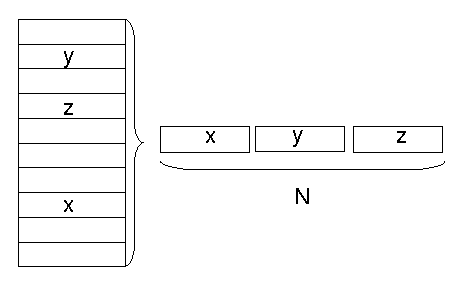
\includegraphics[width=2.5in]{full}
\caption{Fully N-associative cache} \label{full_assoc}
\end{figure}

\emph{Fully N-associative cache} consists of N cells (N means
\emph{cache associativity}). Each cache cell may store data from any
memory cell. All cache cells correspond to the different memory
cells. Access to memory starts from access to cache. Search data in
cache performs for each cache cells in parallel. \emph{Cache hit}
means existence data in cache. \emph{Cache miss} means absence of
data in cache. In case of cache miss one cache cell must be replaced
on data from required address by specific \emph{replacement
strategy}. This paper uses LRU replacement strategy (Least Recently
Used). According to LRU the least recently used cache cell will be
evicted. At the following phrase "evicted address $x$" means evicted
data by address $x$.

Proposed algorithm based on the following properties of evicted
addresses:
\begin{enumerate}
\item any evicted address was inserted by instruction from test template
with cache miss or was in the initial contents of cache;
\item between replacing and the last access to the same address
(cache hit or cache miss) there are accesses to the whole cache
without address itself.
\end{enumerate}

Proposed algorithm generates constraints on the following variables:
\begin{enumerate}
\item $\alpha_1, \alpha_2, ...,\alpha_N$ --  initial contents of cache
(its count equals to cache associativity);
\item hits-addresses (addresses of instructions from test templates
with cache hit test situation);
\item misses-addresses (addresses of instructions from test templates
with cache miss test situation);
\item evicted addresses (evicted addresses of instructions from test templates
with cache miss test situation);
\item $L_0, L_1, ...$ -- cache states
\end{enumerate}

Each instruction from test template with cache hit gives 1 new
variable, and each instruction with cache miss gives 3 new variable
(1 for miss address, 1 for evicted address, and 1 for cache state).
Proposed algorithm generates constraints for each instruction from
test template by the following ($N$ means cache associativity):
\begin{enumerate}
\item "initial constraints" are generated one time for any test template:
$L_0 = \{ \alpha_1, \alpha_2,..., \alpha_N\}$, $|L_0| = N$ (other
words, numbers $\alpha_1, \alpha_2,..., \alpha_N$ are different);
\item "hit-constraints" are generated for each instruction
from test template with cache hit: $x \in L$, when $x$ means address
from instruction, $L$ means a current cache state-variable;
\item "miss-constraints" are generated for each instruction
from test template with cache miss ($x$ means evicting address, $y$
means evicted address, $L$ means a current cache state-variable): $y
\in L, x \notin L, L' = L \cup \{x\} \setminus \{y\}, lru(y)$, $L'$
became a current cache state-variable for the next instruction.
\end{enumerate}

Constraint $lru(y)$ defines $y$ as the least recently used address.

\begin{figure}[h]
\centering
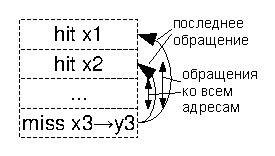
\includegraphics[width=2.5in]{lru}
\caption{LRU} \label{lru_picture}
\end{figure}

Constraint $lru(y)$ is disjunction of constraints corresponded to
cases of the last access to the $y$ before its eviction. Each its
clause is conjunction of the following constraints ($x$ means the
address-variable from the last access to the $y$):
\begin{enumerate}
\item $x = y$
\item $ L \setminus \{y\} = \{ x_1, x_2, ..., x_n \}$, where $x_1, x_2, ...,
x_n$ are all addresses accessed between accesses to $x$ and $y$
(hits and misses).
\end{enumerate}

The last access to the $y$ can correspond to the previous
instruction of test template or to the cell from initial cache
state.

Consider an example of test template and its test data generation
for 3-associative cache.

LOAD x, y @ Hit

STORE u, z @ Miss

LOAD z, y @ Hit

Define unique names for variables in test template (each new
variable shouldn't change its value). LOAD gives new version for its
first argument. STORE doesn't generate new version of variables.
Define new variable $z'_0$ for evicted address from the second
instruction (this variable won't be included to the solution):

LOAD $x_1, y_0$ @ Hit

STORE $u_0, z_0$ @ Miss $\rightarrow z'_0$

LOAD $z_1, y_0$ @ Hit

Define variables for initial contents of cache: $\{ \alpha, \beta,
\gamma \}$ (its count equals to cache associativity).

So the task is looking for values of $x_0, y_0, z_0, u_0, \alpha,
\beta, \gamma$ according to test template. This task has more than 1
solutions. But any solution is enough.

The first constraints describe cache hits and misses as belong to
the current state of cache:

$y_0 \in \{ \alpha, \beta, \gamma \}$,

$z_0 \notin \{ \alpha, \beta, \gamma \}$,

$z'_0 \in \{ \alpha, \beta, \gamma \}$,

$y_0 \in \{ \alpha, \beta, \gamma \} \setminus \{z'_0 \} \cup \{ z_0
\}$,

$\alpha, \beta, \gamma$ -- different

Define constraint $lru(z'_0)$. Candidates of the last access to the
this address are $y_0, \gamma, \beta, \alpha$. The first and the
second candidates aren't suitable because constraint $L\setminus \{
z'_0\} = X$ is false because of different compared sets capacity.
Remainder candidates give the following disjunction:

$z'_0 = \beta \wedge \{ \alpha, \beta, \gamma \} \setminus \{z'_0 \}
= \{ \gamma, y_0 \}$

$\vee$

$z'_0 = \alpha \wedge \{ \alpha, \beta, \gamma \} \setminus \{z'_0
\} = \{ \beta, \gamma, y_0 \}$

Simplify it:

$z'_0 = \beta \wedge \{ \alpha, \gamma \} = \{ \gamma, y_0 \}$

$\vee$

$z'_0 = \alpha \wedge \{ \beta, \gamma \} = \{ \beta, \gamma, y_0
\}$

Further simplify:

$z'_0 = \beta \wedge y_0 = \alpha$

$\vee$

$z'_0 = \alpha \wedge y_0 \in \{ \beta, \gamma \}$

Consider the first clause with the rest of constraints (variable
$z'_0$ isn't needed in solution):

$y_0 = \alpha$

$z_0 \notin \{ \alpha, \beta, \gamma \}$,

$\alpha, \beta, \gamma$ -- different

Note that $x_0$ and $u_0$ don't take part in constraints. So their
values may be arbitrary.

Lets bit length of addresses is 8. So domain of all
variable-addresses is from 0 to 255. Satisfying constraints
variables can get the following values (these values are not
unique):

$\alpha = y_0 = x_0 = u_0 = 0$

$\beta = 1$

$\gamma = 2$

$z_0 = 3$

Verify test template execution with computed initial cache state and
register values:

initial cache state is [2, 1, 0]

LOAD x, 0 - Hit, because 0 $\in \{2,1,0\}$; according to LRU the
next cache state is [0, 2, 1]

STORE 0, 3 - Miss, because 3 $\notin \{0,2,1\}$; according to LRU 3
goes to cache, 1 is evicted from cache, the next cache state is [3,
0, 2]

LOAD z, 0 - Hit, because 0 $\in \{3, 0, 2\}$

All instructions from test template were executed according to given
test situations.
